\chapter{Hardware Design and Development of an Integrated Mobile Platform}
\label{cha:Platform }


\begin{figure}
\centering
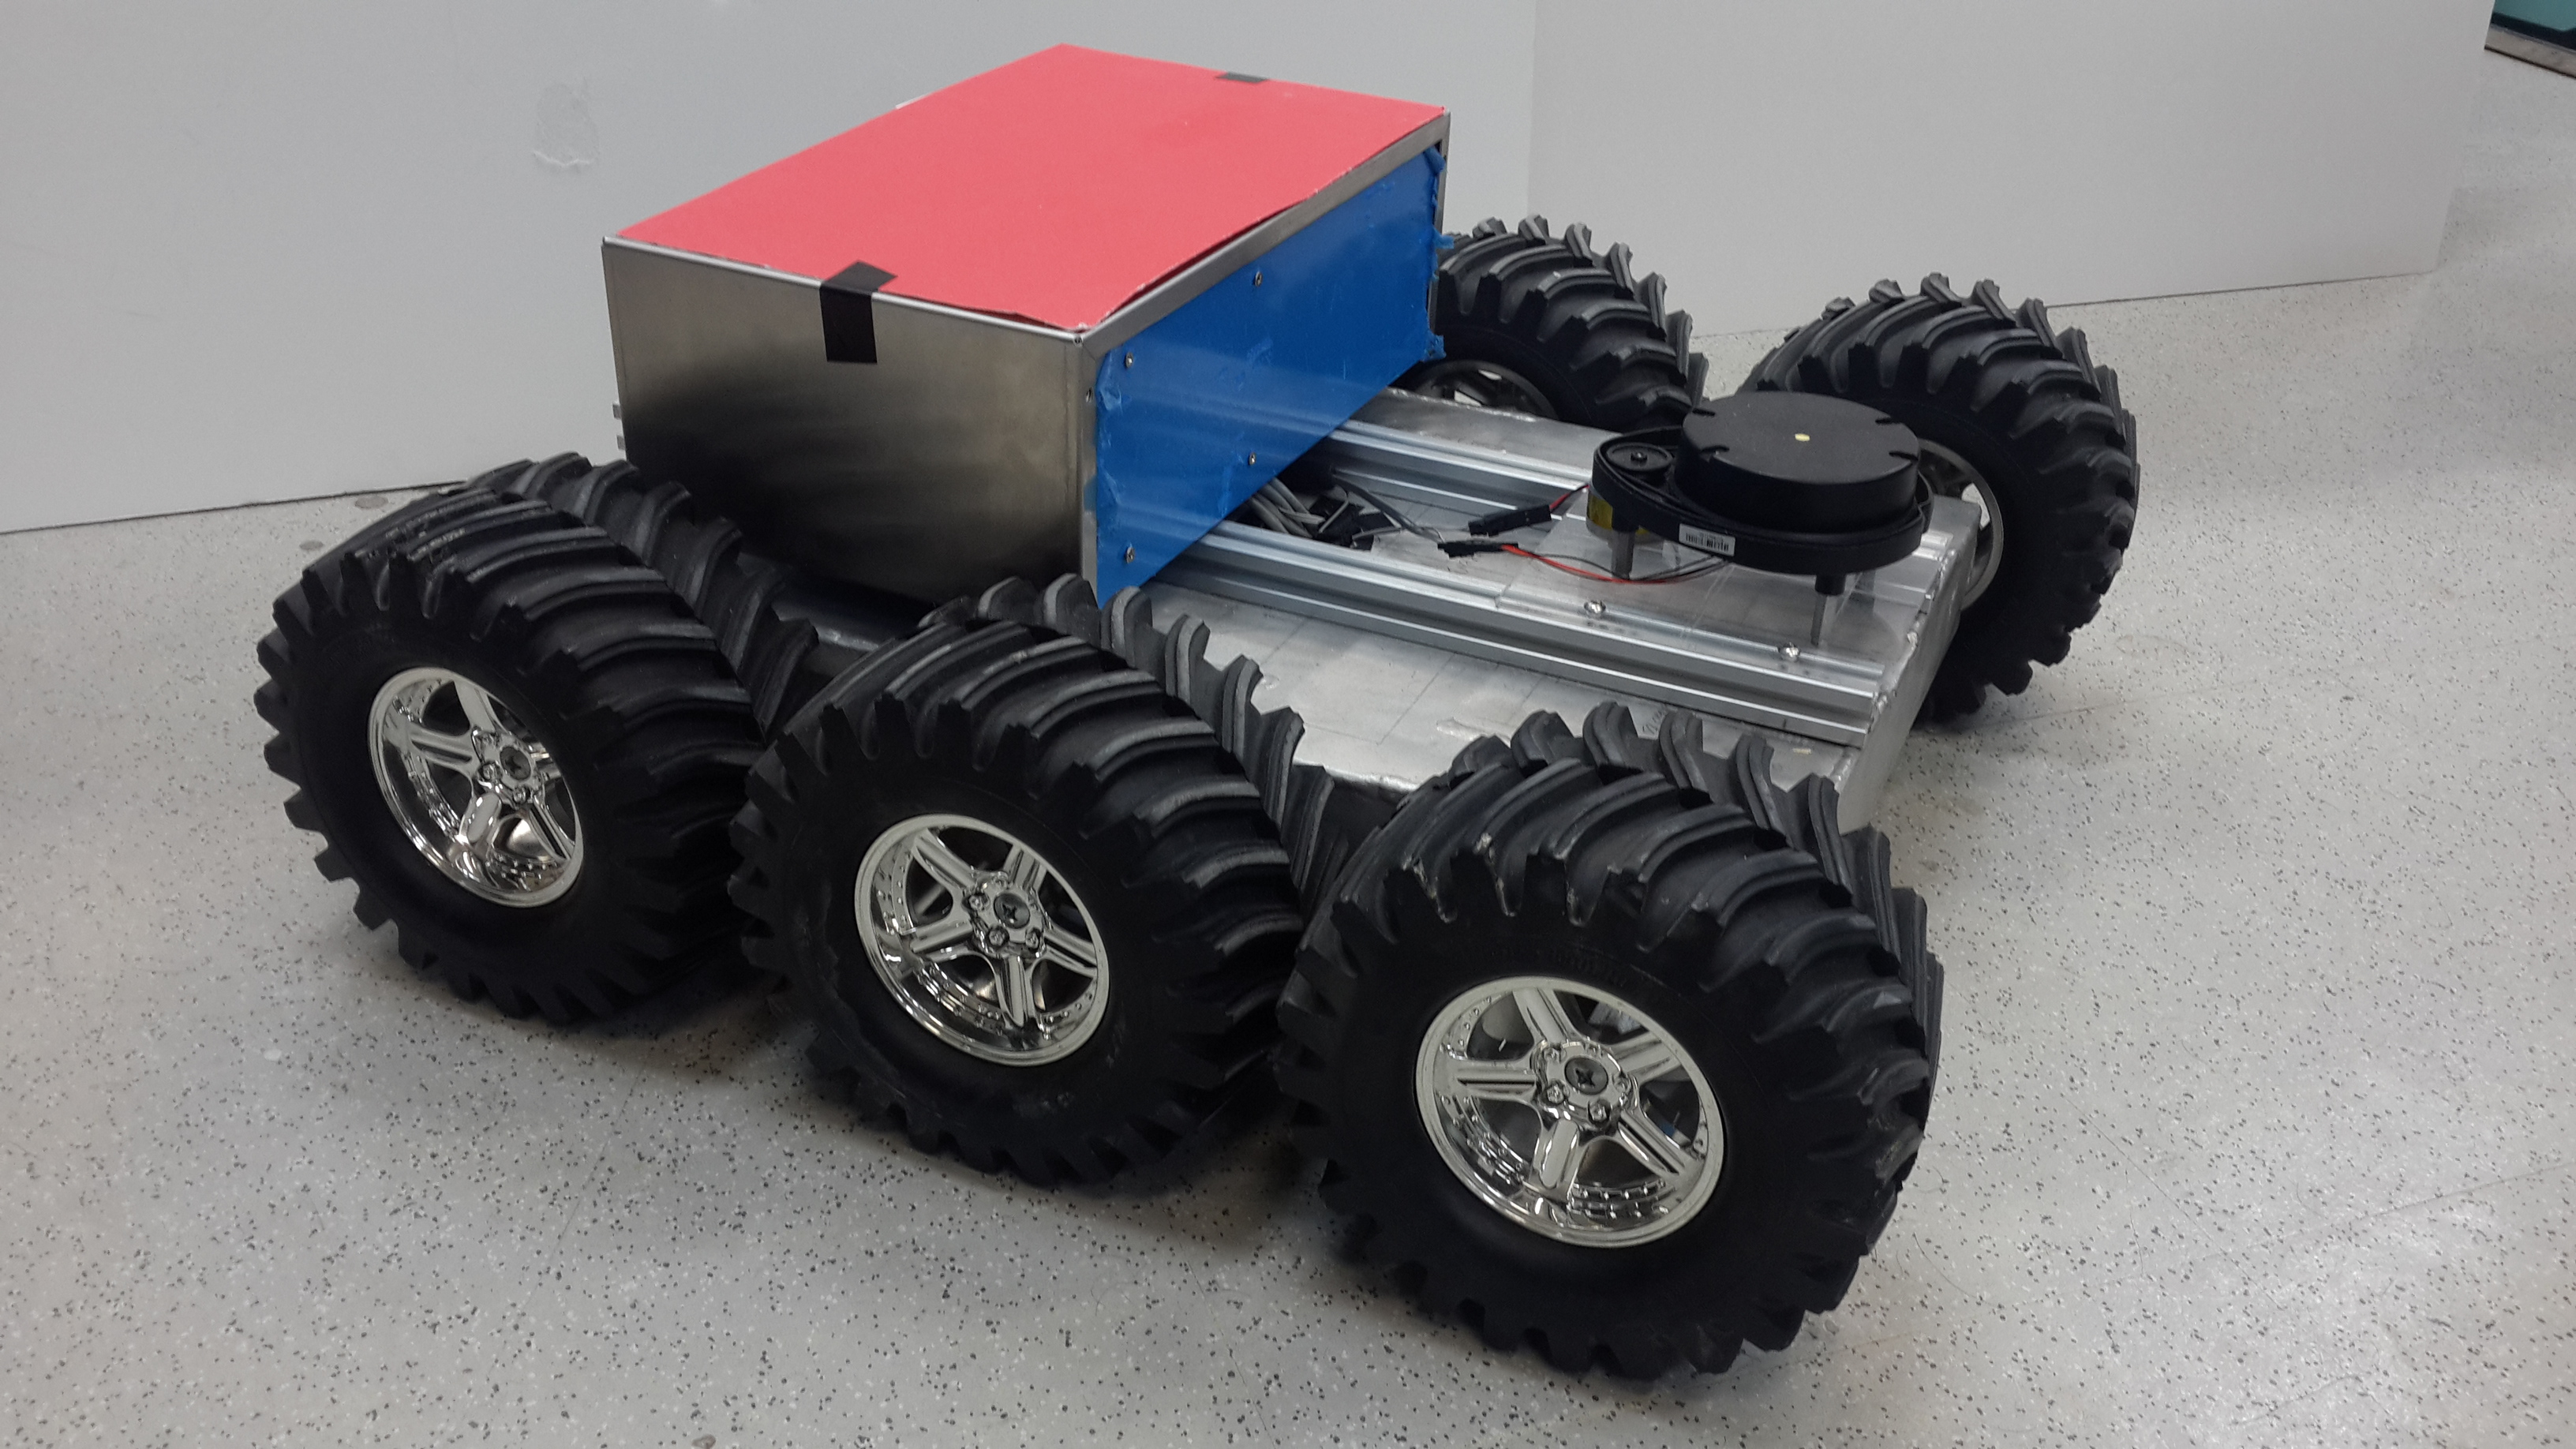
\includegraphics[width=0.5\textwidth]{IMP_color}
\caption{The Integrated Mobile Platform.}
\label{fig:IMP_color}
\end{figure}
\section{Overview and Design Goals}

The Integrated Mobile Platform (IMP) is designed as a robust, scalable platform for Simultaneous Localization and Mapping in a variety of complex environments along with capability for autonomous navigation and decision making. IMP is designed as a platform that can be used both for deployment as well as research. Hence, modularity is emphasized in its design. 

For the primary purpose of SLAM, the major requirements of such a platform are:
\begin{description}
	\item[Mobility] Has to be able to move with a variety of speeds and relatively small turning radii as it is to be used indoors. 
	\item[Self-position acknowledgment] Has to have proprioceptive sensors which give an estimate of its own position and orientation.
	\item[Environment sensing] Has to have sensors to perceive the environment. 
	\item[On-board computational power] Has to have sufficient on-board processing power to do the computations necessary for SLAM and other navigation and obstacle detection algorithms.
	\item[Real-time controller] Has to be capable of real time control implementation.
	\item[Communication] Has to have robust communication between the different components and also with the ground station. 
	\item[Memory] Has to have sufficient on-board memory to collect data to enable testing of SLAM algorithms off-line.  
	\item[Modularity] The various components, both hardware and software, need to be designed in such a way that they are swappable with other components.
	\item[Payload Capacity] The platform has to be capable of carrying sufficient payload for both sensory components and for any applications it is deployed for.
\end{description}

While these requirements define the bare minimum that is needed for such a platform, the design goals that guided the development of IMP were broader. The design goals were as follows:

\begin{itemize}
	\item Have a hardware design capable of supporting large payloads and which can be scaled for any desired run time.
	\item Have enough computational power for implementing real time algorithms for autonomy.
	\item Design modular hardware and software interfaces for the sensors to allow testing of different sensors and sensor fusion algorithms.
\end{itemize}

With these goals in mind, the IMP was designed as a six wheeled differential drive platform with a multi-processor control system, including two micro-controllers and a single-board computer. The platform was also equipped with a number of sensors: 1)~a scanning laser range finder, and 2)~a monocular camera. Additionally two of the platform wheels are equipped with encoders and the embedded processor module is equipped with an Inertial Measurement Unit (IMU). 

The following section discusses the design process involved and the resulting features of IMP, with respect to the hardware components and with respect to the major sensory, computational and power handling components of IMP. The communication and information flow in the current implementation of using IMP for data collection for SLAM is then discussed. The motion model for EKF SLAM using this platform is discussed in the last section. 

\section{Mechanical Design}

The first design decision was the basic configuration of the robot. The primary motivation being simplicity, the type of robot was decided to be a differential drive robot, which is a mobile robot whose movement is based on at least two separately driven wheels placed on either side of the robot body. Therefore the IMP can change its direction by varying the relative rate of rotation of its wheels and hence does not require an additional steering mechanism. If both the wheels are driven in the same direction and speed, the robot will go forward in a straight line. If both wheels are turned with equal speed in opposite directions, the robot will rotate about the central point of the platform axes. Differential drive system  has several advantages over other systems. Ackerman steering, which is used in automobiles, has a lower bound on the turning radius and also requires additional control inputs for steering. In other systems such as tank treads, it is difficult to reconstruct the odometry; as the target of the robot is autonomy, this proves to be a disadvantage. A differential drive robot gives on the spot turning capability with minimal control complexity.

\begin{figure}
    \centering
    \begin{subfigure}[b]{0.3\textwidth}
	    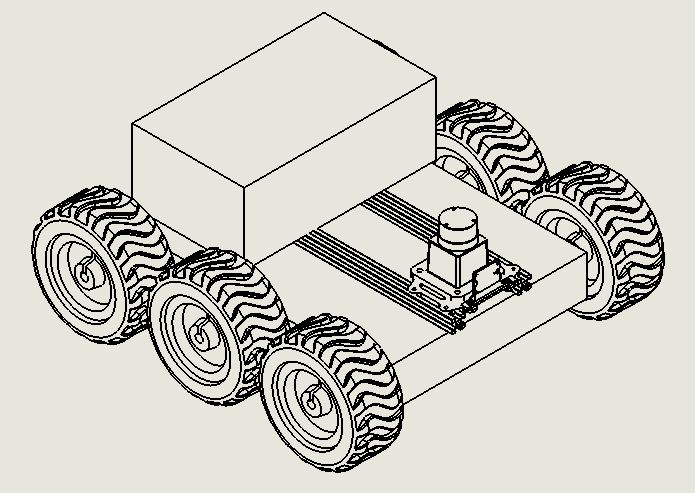
\includegraphics[width=\textwidth]{IMP}
	    \caption{Isometric view.}
	    \label{fig:IMP}
    \end{subfigure}
    \quad %add desired spacing between images, e. g. ~, \quad, \qquad, \hfill etc.
      %(or a blank line to force the subfigure onto a new line)
    \begin{subfigure}[b]{0.3\textwidth}
        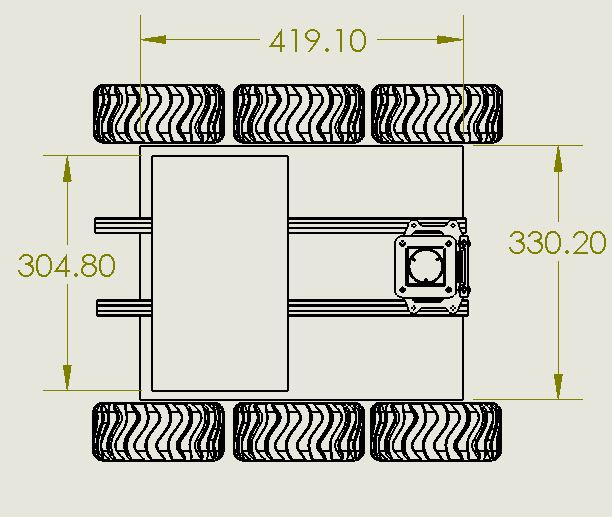
\includegraphics[width=\textwidth]{IMPtop}
        \caption{Top view.}
        \label{fig:IMPtop}
    \end{subfigure}%
    \quad %add desired spacing between images, e. g. ~, \quad, \qquad, \hfill etc.
      %(or a blank line to force the subfigure onto a new line)
    \begin{subfigure}[b]{0.3\textwidth}
        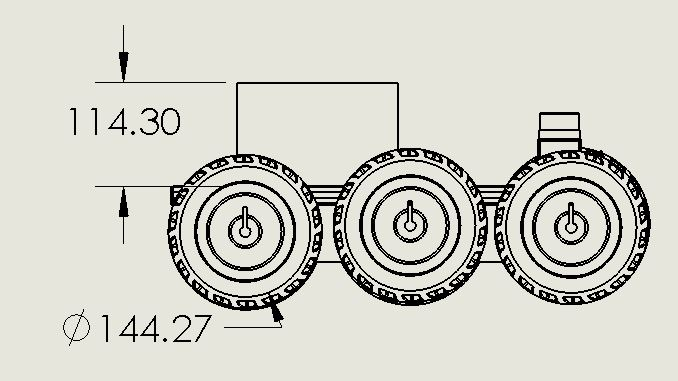
\includegraphics[width=\textwidth]{IMPside}
        \caption{Side view.}
        \label{fig:IMPside}
    \end{subfigure}%
    \caption{Dimensions of \imp.}
    \label{fig:IMPviews}
\end{figure}

Once the type of robot was decided, the next important consideration was its size. This mainly depends on the budget and the application the robot is being built for. As per the design principles stated, the primary objective is to keep the robot scalable, and equipped to carry larger payloads. Thus, the slightly larger size of the robot will allow payloads to be attached in the future. The dimensions of the robot are shown in Figure~\ref{fig:IMPviews}. The chassis is designed to be lightweight but structurally sound so as to allow larger payload capability. For this purpose the material of choice is aluminum which has the structural strength required. The chassis structure itself is a hollow cuboid, but there are multiple support struts running across its breadth to give added structural strength. This design allows the weight of the chassis to be reduced to about 2.2 kg.

The guiding principle behind the design of the robot was versatility. Therefore, the wheels were chosen to be made of rubber with an offset-V tread to have sufficient friction to traverse both indoor and outdoor environments. The wheel size was chosen based on the size of platform. The number of wheels were picked based on stability, control and sensing requirement. The four outer wheels are driven by DC geared motors generating sufficient torque the robot to have a small turning radius. Putting the encoders on the driven wheels will give errors in odometry when there is slipping of the wheels because of friction loss which is a common occurrence on gravel in outdoor environments and on smooth floors indoors. Due to this the two middle passive wheels were added, which are used for odometry. The passive middle wheels are rotated solely due to the robot motion. Hence, measuring the rotation of the passive wheels yields a more accurate position estimate it gives a better estimate of the path followed by the robot which gives a huge benefit, for autonomous applications. 

Once the basic platform is designed, the choice of motors and battery is a combined decision; the torque capacity of the motors depend mainly on the weight of the payload that is to be carried by the robot. Motors with higher torque capacity draw more current; this in turn demands larger and heavier batteries to achieve consistent runtime. For example, in a previous version, the same platform had a 24V nickel-metal hydride(Ni-MH) battery and DC geared motors with a rated torque of 1.4 kgf-cm. A typical Ni-Mh battery has a specific energy of 20-120 Wh/kg and the result of the heavy payload it was found that the motors were not strong enough to turn the platform itself with a reasonable turn radius. This was due to a combination of both the large weight of the battery and the low torque of the motor. 
%a battery which had an energy rating of 100 Wh, weighed around 1.5 kg. With this configuration,
Both the batteries and the motors were then upgraded, to enable the platform to carry not only its own weight but also additional sensor and computational payloads. Ni-MH batteries were replaced by high specific energy lithium polymer(LiPo) batteries. These batteries typically have a specific energy of 100-265 Wh/kg. The low weight allows for installation of additional battery capacity without having to change the motors if needed. The motors currently used on the \imp have a rated load of 7.3 kgf-cm, which makes the IMP ideal for larger payloads and on-spot turning..

%The battery used on IMP with around 27 Wh, weighs around 0.4 kg

%As seem in Figure~\ref{fig:IMP_color} and~\ref{fig:IMP}, the rest of the components on IMP are attached using an aluminum channel as shown in Figure~\ref{fig:mounting} and not welded. This allows for easy switching during further expansion. The Sensors are also mounted using 3D printed modular mounts as in Figure~\ref{fig:modular_hokuyoBase}.
%
%\begin{figure}
%    \centering
%    \begin{subfigure}[b]{0.4\textwidth}
%		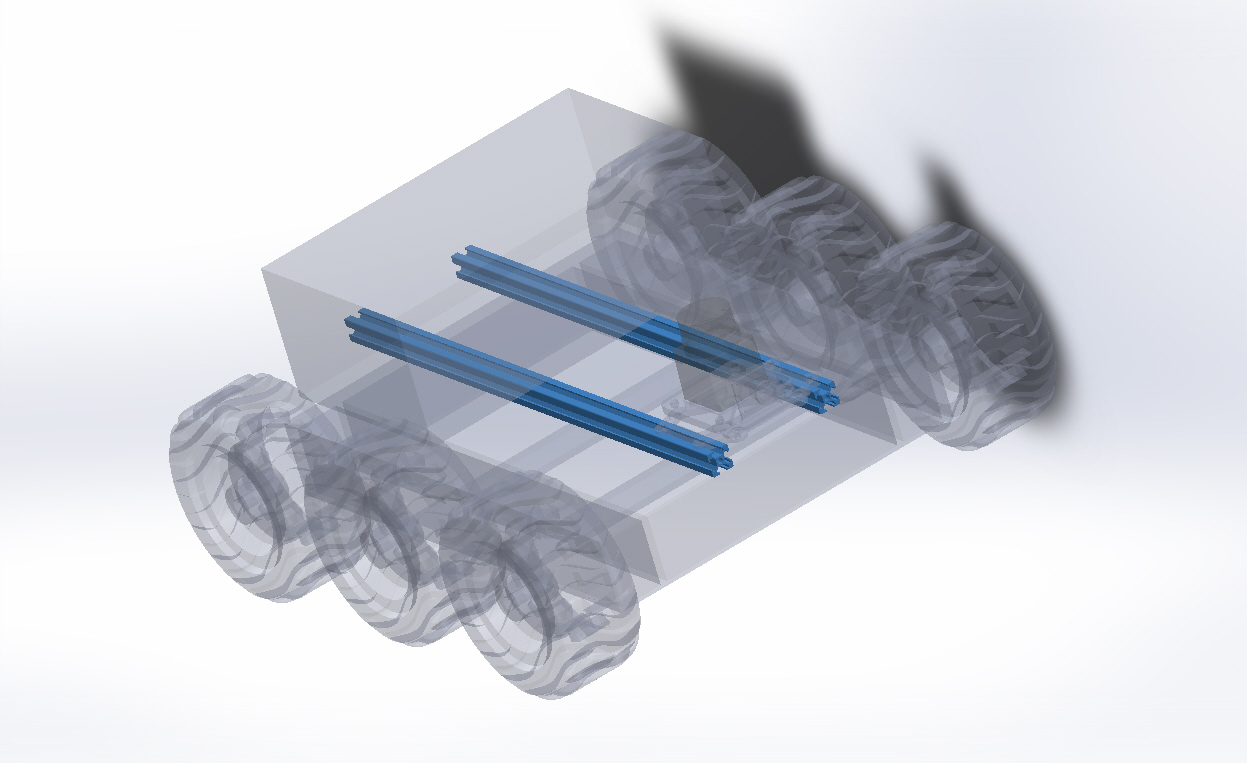
\includegraphics[width=\textwidth]{beams}
%		\caption{Mounting rails on IMP}
%		\label{fig:mounting}
%    \end{subfigure}
%    \qquad %add desired spacing between images, e. g. ~, \quad, \qquad, \hfill etc.
%      %(or a blank line to force the subfigure onto a new line)
%    \begin{subfigure}[b]{0.4\textwidth}
%        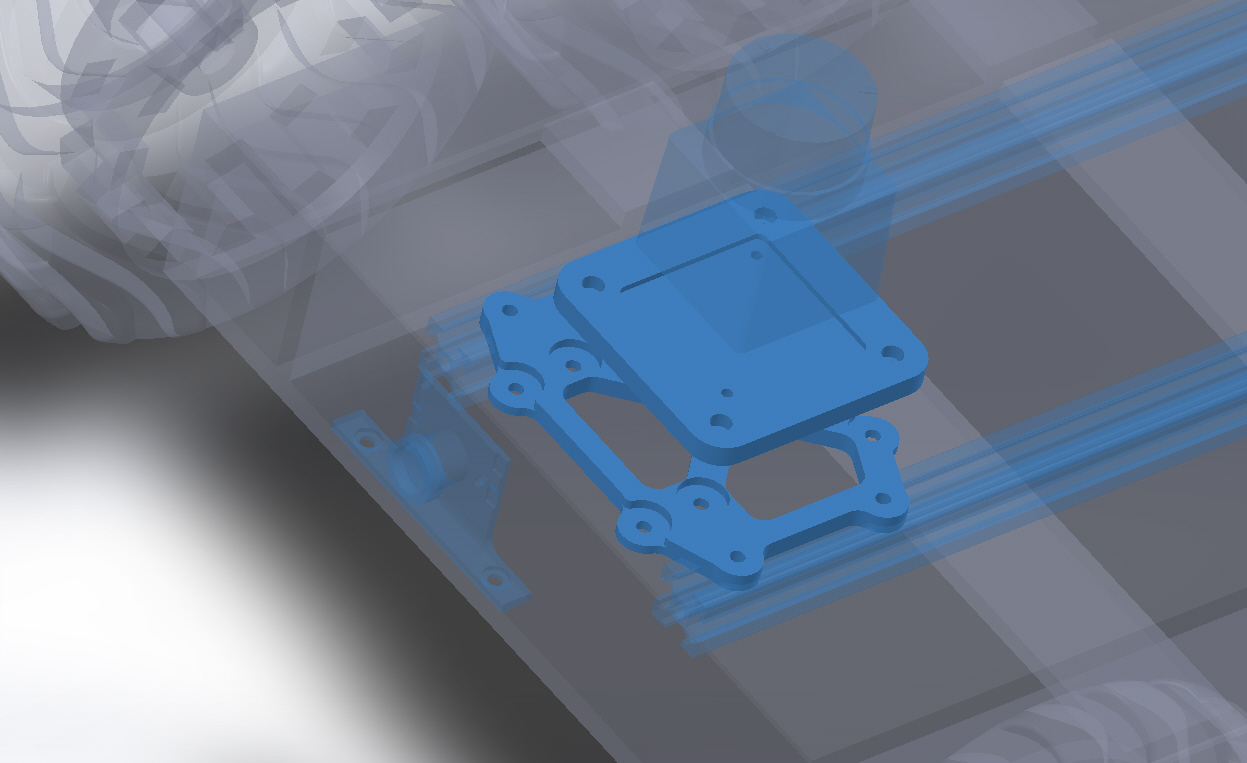
\includegraphics[width=\textwidth]{modular_hokuyoBase}
%        \caption{Mounting plates for sensors}
%        \label{fig:modular_hokuyoBase}
%    \end{subfigure}
%    \caption{Modular design of IMP}
%    \label{fig: Modular}
%\end{figure}

\section{Electrical Subsystem}

The electrical design is guided by the same principles of scalability for autonomy, and flexibility. The major computational and sensory payloads on the IMP are:

\begin{itemize}
\item 	Dual processor AutoPilot unit with a 9-axis inertial measurement unit.
\item  	ODROID-XU single-board computer.
\item 	MA 3 miniature absolute magnetic shaft encoders.
\item  	\textit{Leopard Imaging} 5 MP camera.
\item  	Hokuyo-URG-04lx scanning LIDAR .
\item	TP-Link Nano wireless module
\item  	XBEE wireless radio
\end{itemize}
\begin{figure}
\centering
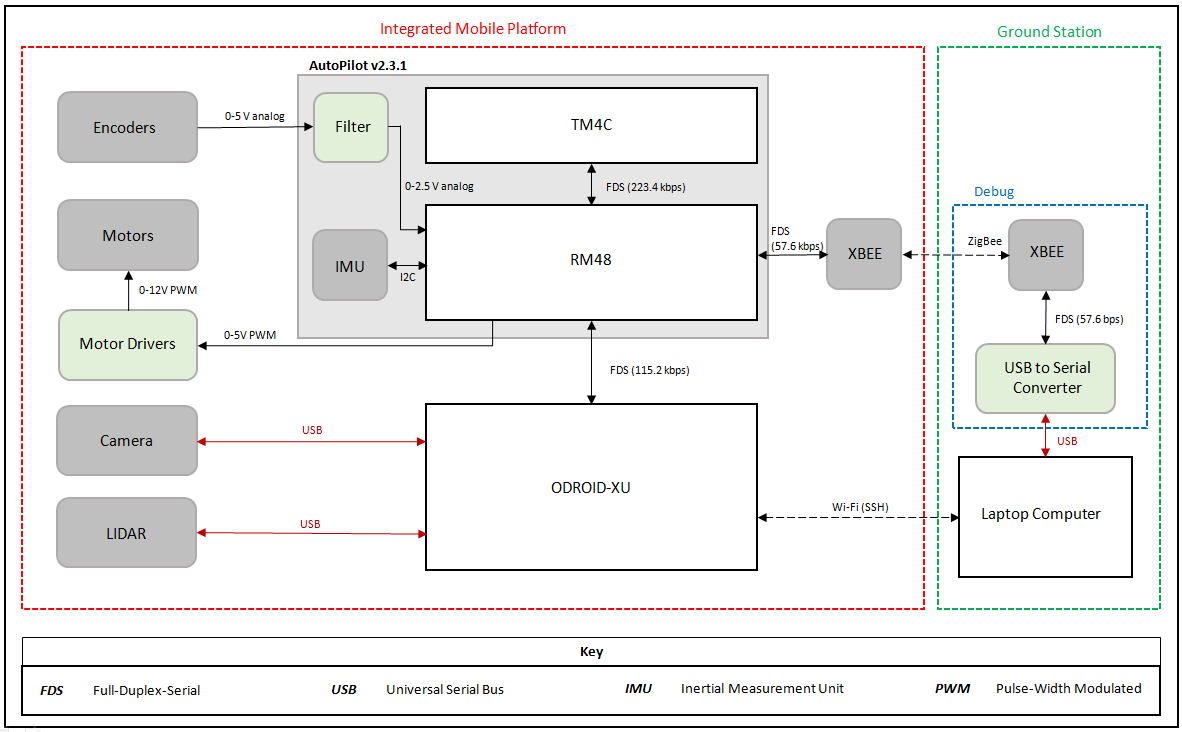
\includegraphics[width = \textwidth]{system_diagram}
\caption{System diagram of \imp.}
\label{fig:system_digram}
\end{figure}


\subsection{Device Purpose and Descriptions}

\begin{figure}
\centering
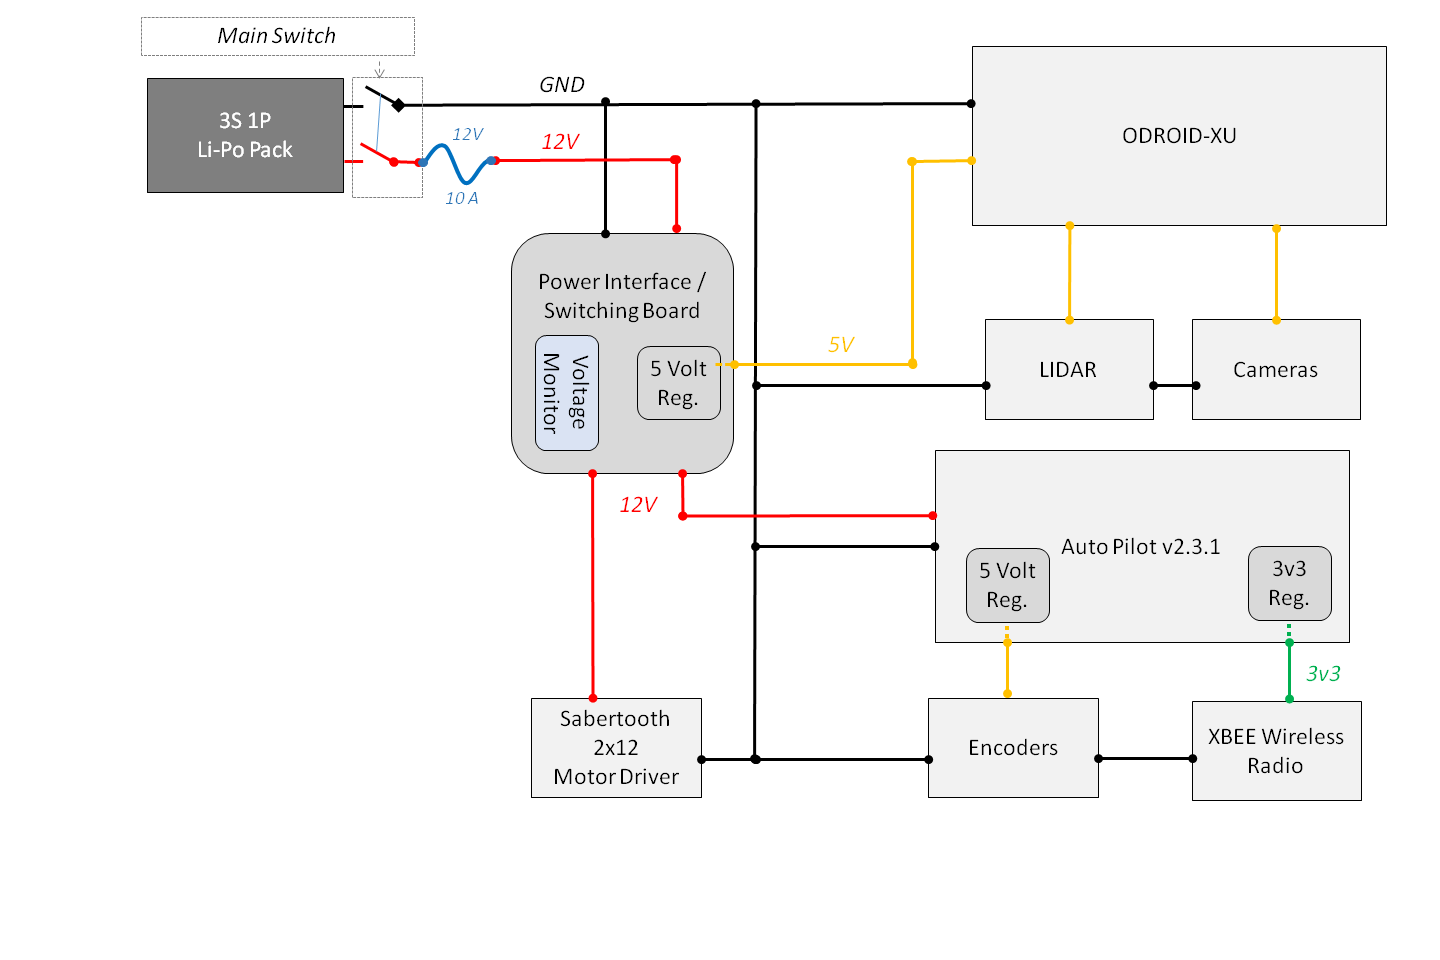
\includegraphics[width = \textwidth]{power_diagram}
\caption{\imp Power routing diagram.}
\label{fig:power_diagram}
\end{figure}

\subsubsection{AutoPilot}

The AutoPilot is a dual processor unit that is equipped for low level real-time control algorithms as well to act as a data acquisition platform and an input/output interface for the robot. The AutoPilot consists of two processing units: a Texas Instruments TM4C and a RM48 ARM micro-controller (MCU), which operate at 80 MHz and 220 MHz, respectively. These processors can communicate with each other either over UART or Controller Area Network(CAN). One UART of the RM48 MCU is also connected to an on-board computer, an ODROID-XU through a level translator circuit. The AutoPilot is powered via an external 12 V supply. This AutoPilot unit includes a 9-axis inertial measurement unit (IMU) which consists of two, 3-axis accelerometers, one 3-axis rate gyro, and a 3-axis magnetometer unit. Additionally, the AutoPilot includes humidity and temperature sensors and can be easily interfaced to a GPS unit.

The AutoPilot being a versatile device can be used for a large number of purposes depending on the implementation. A part of the autonomy algorithm can be off loaded to the AutoPilot, or low level real-time control algorithms such as PID can be implemented. The autopilot is currently implemented as an I/o processing and sensor data acquisition unit and is interfaced with the encoders, the IMU and the motor driver.

\begin{figure}
\centering
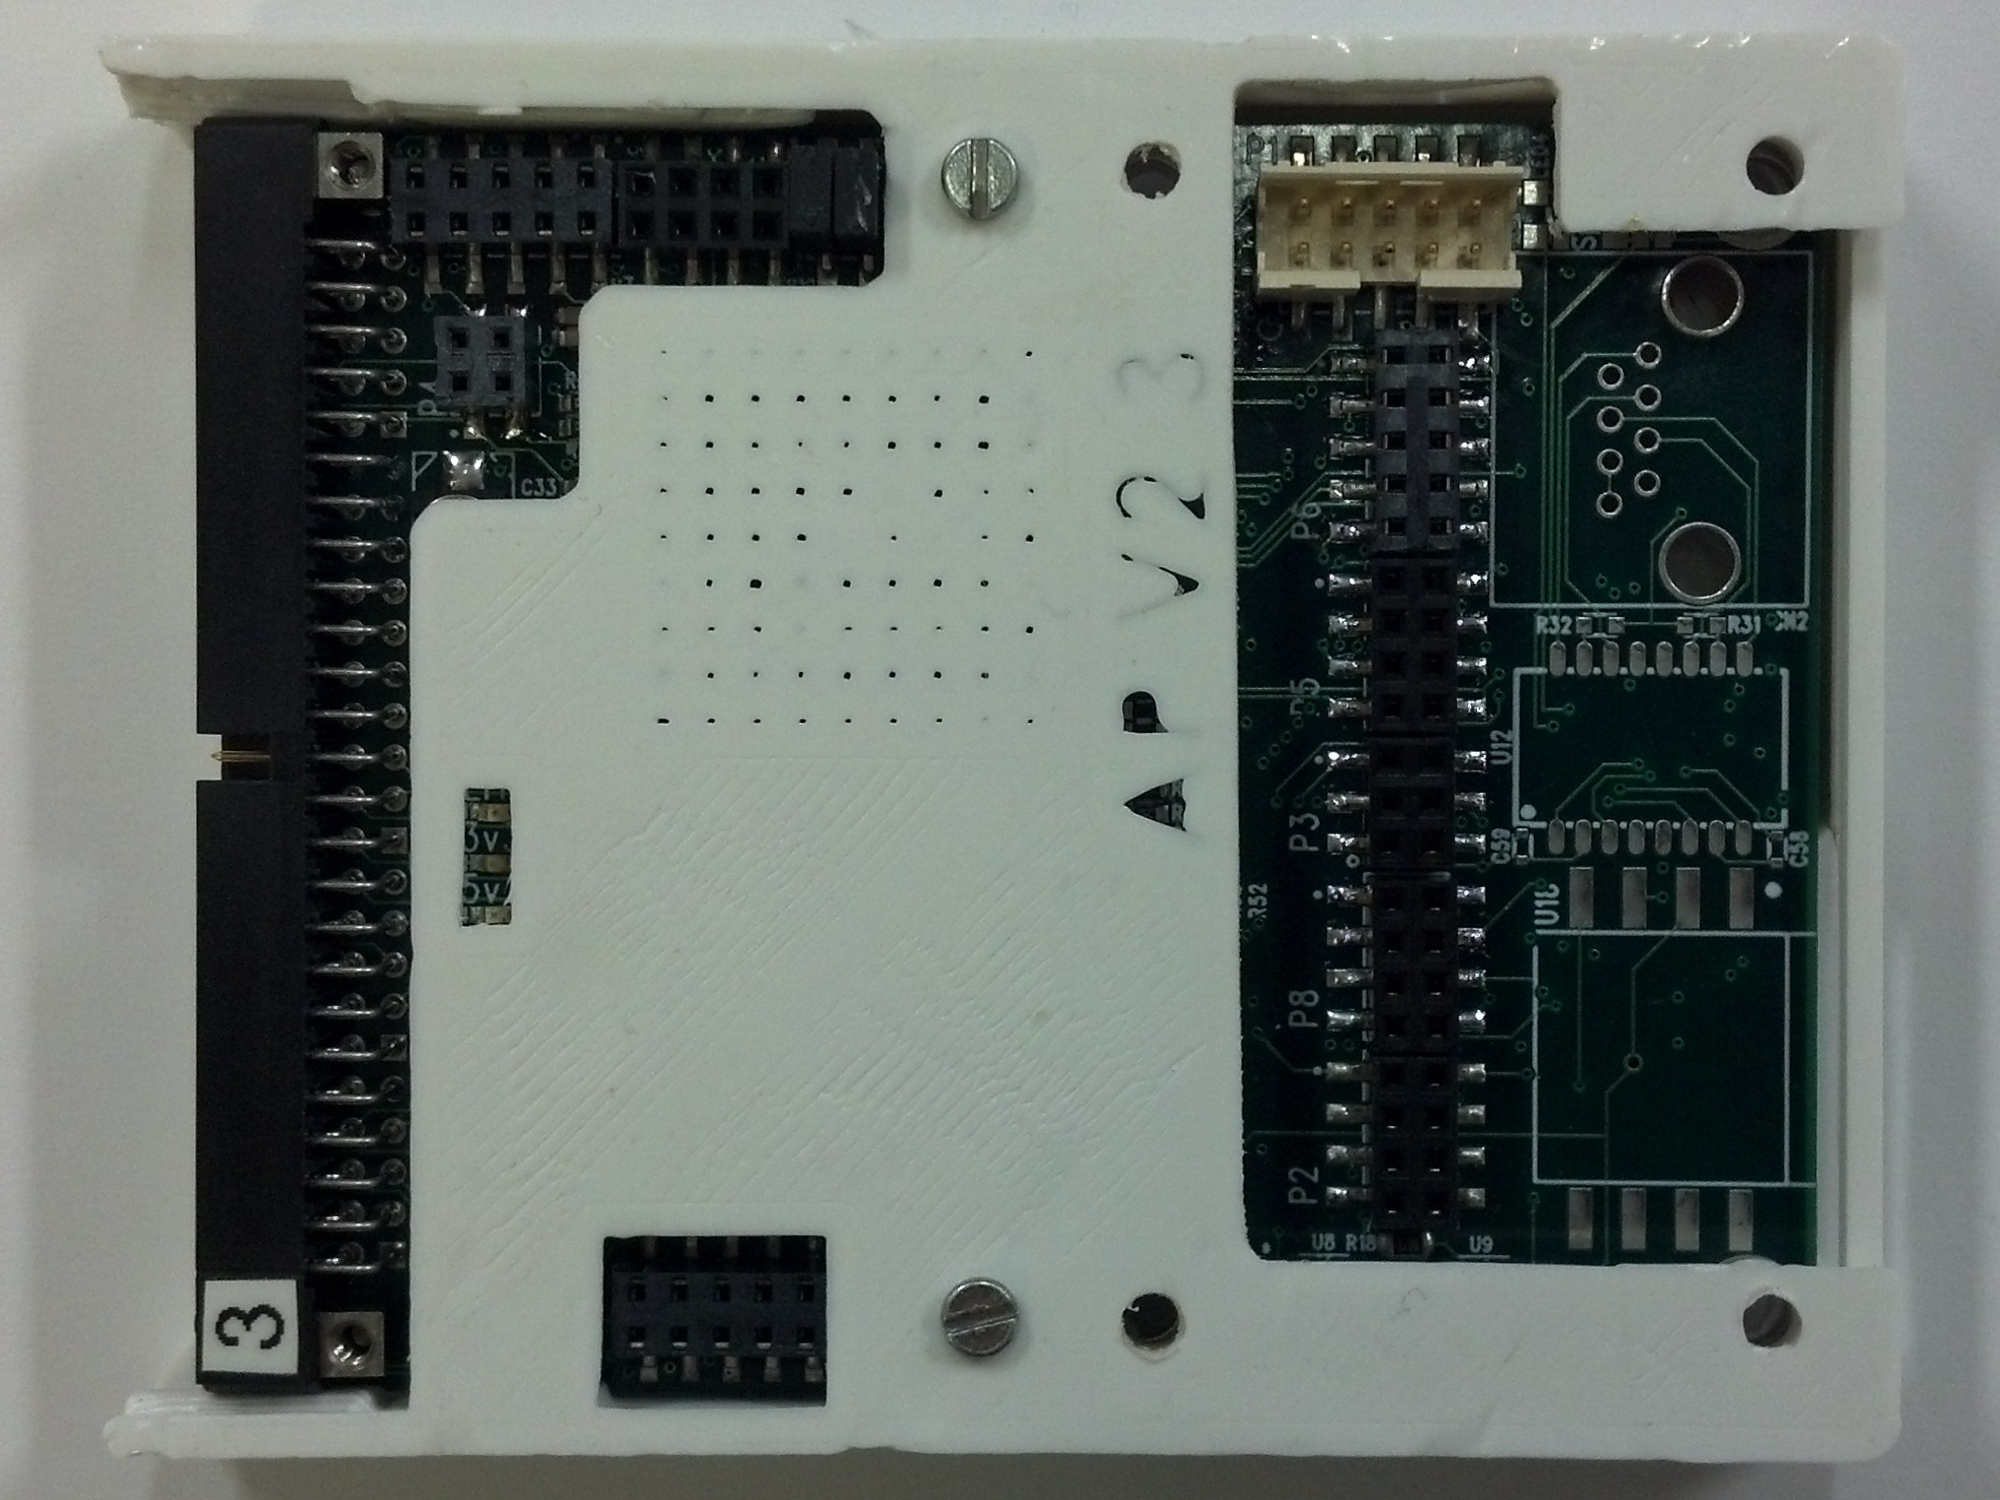
\includegraphics[width=0.5\textwidth]{APTop1}
\caption{Autopilot on the \imp.}
\label{fig:APTop1}
\end{figure}

\subsubsection{ODROID XU}

The ODROID is the on-board computer and provides significant computational power especially when the IMP is used for real time autonomous navigation. Equipped with Samsung Exynos5422 Cortex™-A15 2.0Ghz quad core and Cortex™-A7 quad core CPUs the odroid has 2Gbyte LPDDR3 RAM capable of operating at 933MHz and several USB 2 and USB 3 ports for interfacing. With these features, considerably powerful and computationally intensive algorithms for \slam ~along with path planning and decision making can be run. The on-board computer is implemented as a higher level controller of the robot and is powered by a separate 5V regulator as shown in Figure~\ref{fig:power_diagram}.

\begin{figure}[h!]
\centering
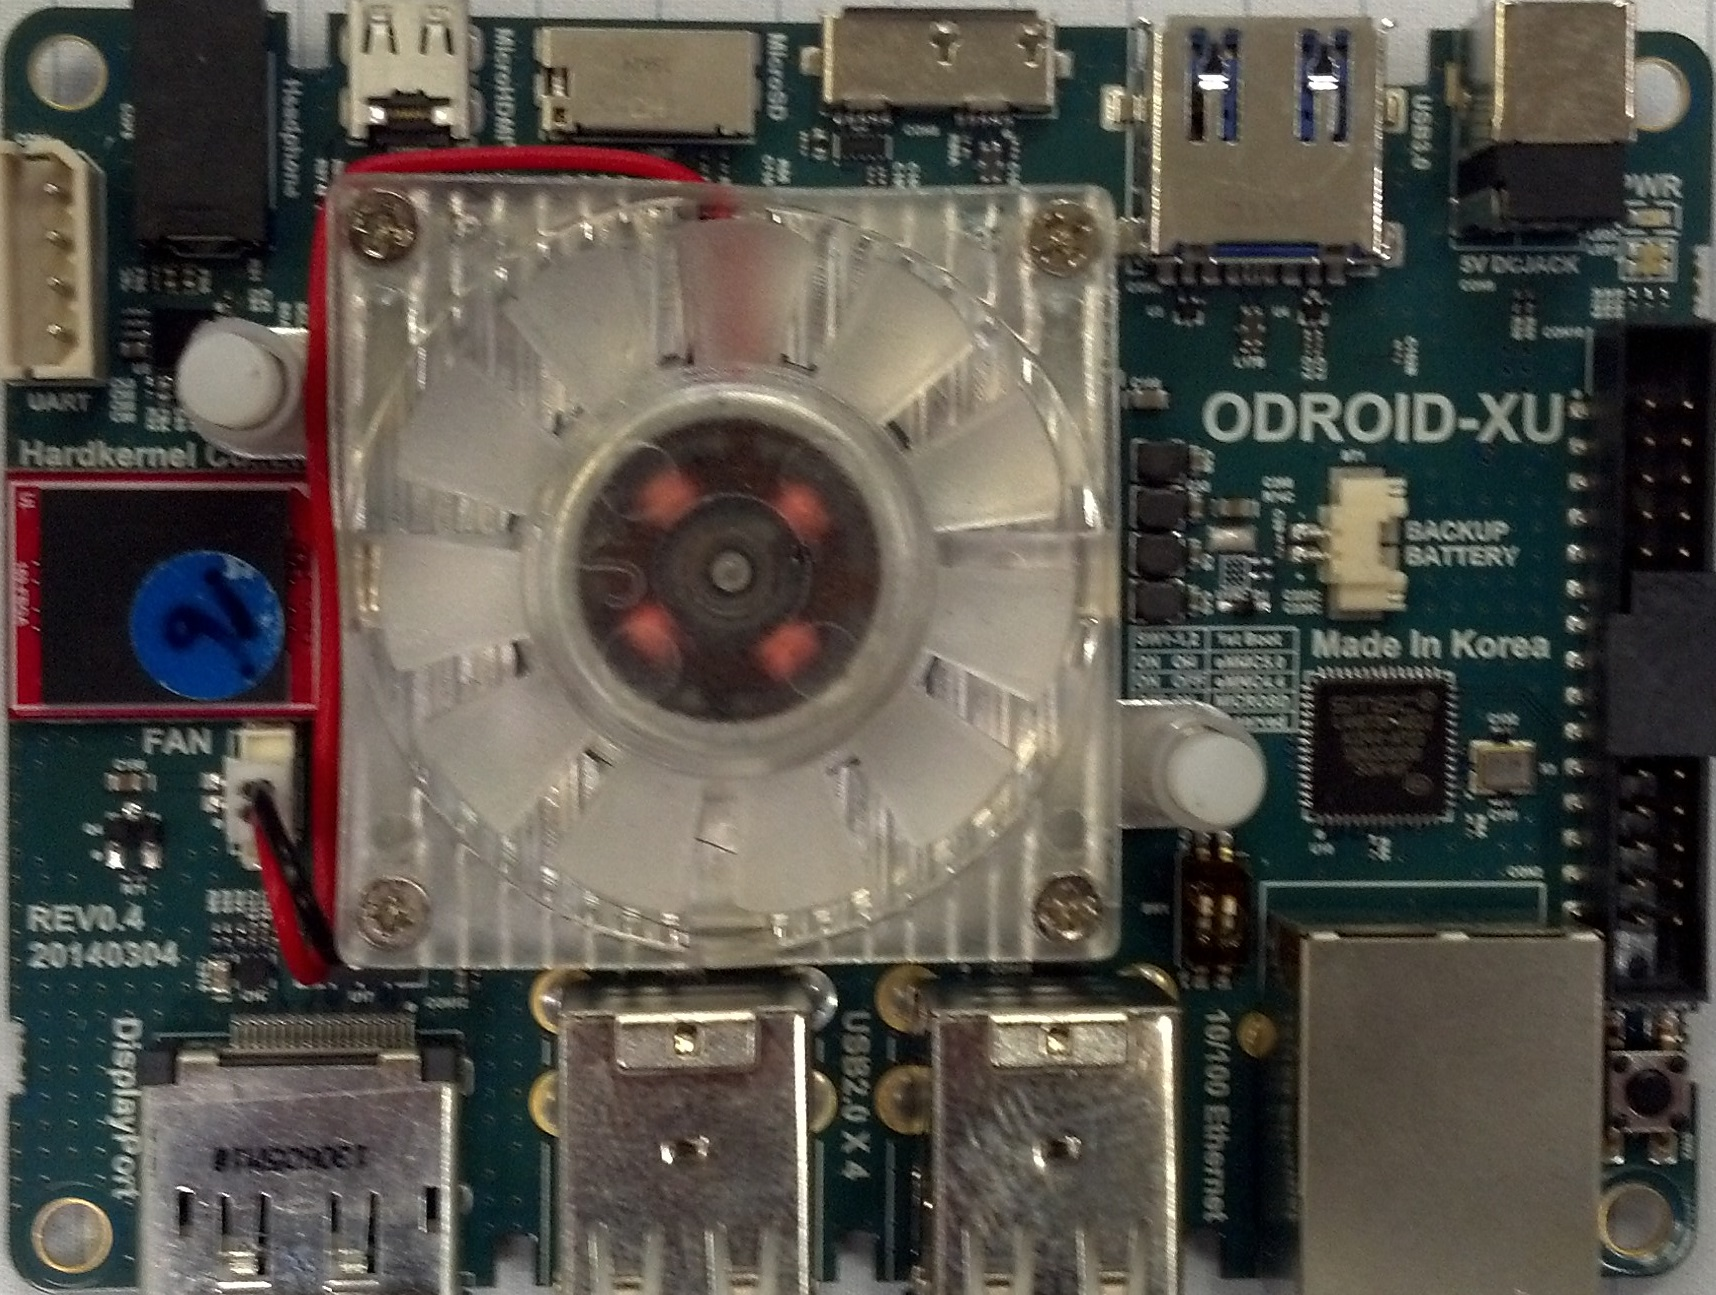
\includegraphics[width=0.5\textwidth]{odroidTop1}
	\caption{Odroid on the \imp.}
	\label{fig:odroidTop1}
\end{figure}

\subsubsection{Encoders}
The magnetic shaft encoders measure the absolute position of the wheel, and provide a 0-5V output and can hence, be modeled as a continuous rotation potentiometer. So while the wheel is continuously turning, the value rises from 0 to 5 volts and then instantaneously drops to 0 at the end of every rotation. Therefore, to calculate rotational speed, the encoder signal has to be first stored in an accumulator and then differentiated. While the signal is reasonably free of noise and performs well for dead reckoning, there exists some component of high frequency noise that needs to be filtered out. So the analog signal is first passed through a hardware based active low pass filter of 950 Hz which is shown in Figure~\ref{fig:low_pass}. A Digital to Analog Converter (DAC) is used to be able to set the reference voltage without having to change the hardware. Both the filter circuit and the DAC are built into the AutoPilot.
\begin{figure}[h]
\centering
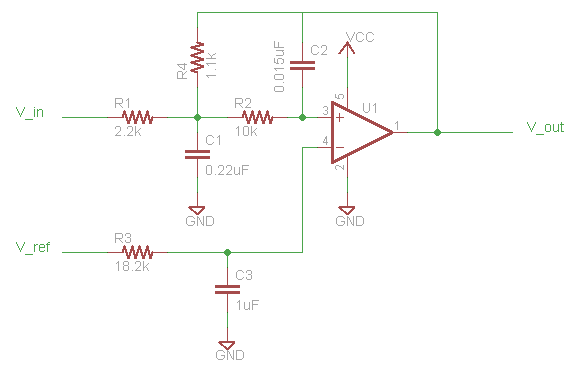
\includegraphics[width=0.5\textwidth]{low_pass}
\caption{Low pass filter for encoder input.}
\label{fig:low_pass}
\end{figure}
\subsubsection{Camera}

The camera can be used for sensing features in the environment, or for visual odometry which gives an estimate of the robot's pose and hence, can act both as an exteroceptive sensor as well as a proprioceptive sensor. This gives a major advantage in situations where the number of sensors neeed to be minimized.

The \textit{Leopard Imaging} camera, captures 5 megapixel HD images at speeds up to 30 frames per second. The camera has a $ 72^\circ $ horizontal field of view, and $ 30^\circ $ vertical. The ODROID is used to read in the camera data through an USB interface.

\subsubsection{LIDAR}
When picking a LIDAR, the choice needs to be made between using 2D or 3D LIDARs. 3D LIDARs have numerous advantages, but the high cost in addition to its weight limits the applications. It is more practical to have a 2D LIDAR initially with scope for further expansion into 3D. A really simple way to implement 2D LIDAR is to mount a single range finder on a rotating platform. That way the cost can be reduced but the resolution and scanning speed are adversely affected. An earlier iteration of IMP, used a Piccolo Laser Scanner, which had an inexpensive laser range finder being rotated at around 15 Hz. The range finder itself, was based on beam deviation rather than \textit{Time of Flight} which made the range measurements slightly inaccurate.

The current LIDAR used is the Hokuyo URG-04LX Scanning Laser Range Finder which has a low scanning period of 100 ms/scan, and is accurate up to 2 mm. With a $ 240^\circ $ field of view and capability to detect distances from 20 mm to 5600 mm, it provides the robot the capability of sensing the environment to a largely accurate extent.

\subsubsection{Communication Modules}
The primary channel of communication is the Wi-Fi module, a TP-Link Nano with a speed of 150 Mbps and is configured in \textit{AP Router} mode. This lets IMP host its own Wi-Fi which is advantageous when IMP is to be used in an environment where there are no existing Wi-Fi networks available. 

Another wireless communication interface is the XBee connected directly to the AutoPilot through a UART port. This can be used if the AutoPilot is to be commanded directly for tele-operation without using the ODROID. In the current configuration Xbee is used as a Debug port so that the status of the AutoPilot can be checked whenever needed. 

\section{Software Design for Data Collection}
The Autopilot has a precise Real Time Interrupt module in the RM48, and therefore maintains a timebase for the whole process. Its interrupts are set in a half millisecond cycles. Every millisecond the encoders are read, and updates an accumulator. The IMU outputs are read every 5 ms. Both the encoder and the IMU data is logged on the SD card at a rate of 80Hz. Every 10 ms, the latest accumulator and IMU readings are sent to the ODROID. 

The ODROID parses the data sent by the AutoPilot. Based on the standard time base, at the rate of 5 Hz, the on-board camera and the LIDAR data are acquired. All the collected data is stored in the file system of the Odroid. These files are then transfered through SSH to the ground station. The ODROID program itself is started and controlled over Wi-Fi, through which the user commands are transmitted. 

\section{Encoder Based Odometry for State Estimate}

The encoders attached on the two passive wheels give an estimate of the robot's movement in each time step. The function used to calculate the robot's movement from the encoder data is the motion model of the robot and is used for equation~\ref{eq:EKF_1} in section~\ref{sec:EKF}. Since this robot has only 3 degrees of freedom, the state vector, $ x \in \Re^3 $, and is defined as $ x = [x,y,\theta]^T $ where $ x $ and $ y $ provide the position of the robot from an arbitrary fixed point in inertial frame of reference. 

\subsection{Motion Model and the Corresponding Differentials}

To estimate the motion model, the left and right wheel movement is first converted into distances traveled through a linear mapping using the known radius of the wheels. These values are represented by $ u = [ l, r ]^T $. The Equations are better implemented as a piecewise function. The two cases of when the robot is estimated to be going straight or to be turning are considered separately. This decision is made by observing the distance traveled by the left and right wheels in the same time step. If they are exactly the same, the robot is assumed to be going straight and the motion model is given by Equation~\ref{eq:Enc_1}.

If $ r = l $,
\begin{equation}
\label{eq:Enc_1}
	\begin{bmatrix}
		\hat{x}^-\\\hat{y}^-\\\hat{\theta}^-
	\end{bmatrix}_k
	=
	\begin{bmatrix}
		\hat{x}\\\hat{y}\\\hat{\theta}
	\end{bmatrix}_{k-1}
	+
	\begin{bmatrix}
		l.\cos(\hat{\theta}_{k-1})\\
		l.\sin(\hat{\theta}_{k-1})\\
		0
	\end{bmatrix}.
\end{equation}
Otherwise, the robot is turning, and Equations~\ref{eq:Enc_2} and~\ref{eq:Enc_3} are used.
			
\begin{figure}
\centering
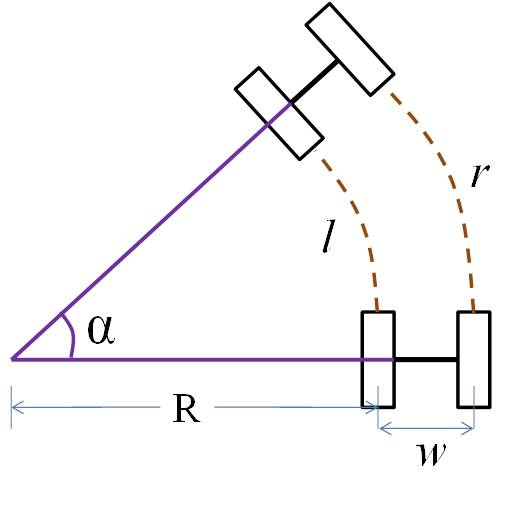
\includegraphics[width=0.3\textwidth,height=0.3\textheight]{differential_turning}
\caption{Motion model of differential drive platform.}
\label{fig:Enc_1}
\end{figure}

If $ r \neq l $,
\begin{equation}
\label{eq:Enc_2}
	\alpha= \frac{r-l}{w}
\qquad
	R=\frac{l}{\alpha}
\end{equation}
\begin{equation}
\label{eq:Enc_3}
	\begin{bmatrix}
		\hat{x}^-\\\hat{y}^-\\\hat{\theta}^-
	\end{bmatrix}_k
	=
	\begin{bmatrix}
		\hat{x}\\\hat{y}\\\hat{\theta}
	\end{bmatrix}_{k-1}
	+
	\begin{bmatrix}
		\left(R+\frac{w}{2}\right)(\sin(\hat{\theta}_{k-1}+\alpha)-\sin(\hat{\theta}_{k-1}))\\
		\left(R+\frac{w}{2}\right)(-\cos(\hat{\theta}_{k-1}+\alpha)-\cos(\hat{\theta}_{k-1}))\\
		\alpha
	\end{bmatrix}
\end{equation}
where $ R,\alpha $ and $ w $ are as shown in Figure~\ref{fig:Enc_1}.

In general, the motion model given by Equations~\ref{eq:Enc_1} to~\ref{eq:Enc_3}, is compactly represented as:
\begin{equation}
\label{eq:Enc_4}
\hat{x}^-_k = f(\hat{x}_{k-1},u_k).
\end{equation}

Once the motion model is known, it is necessary to find its Jacobian with respect to the state. Since both the motion model has 3 dimensions the Jacobian will be a $ 3\times 3 $ matrix given by
\begin{equation}
\label{eq:Enc_5}
A = \frac{\partial f}{\partial x} = 
\begin{bmatrix}
\frac{\partial f_1}{\partial x} & \frac{\partial f_1}{\partial y} & \frac{\partial f_1}{\partial z} \\
\frac{\partial f_2}{\partial x} & \frac{\partial f_2}{\partial y} & \frac{\partial f_2}{\partial z} \\
\frac{\partial f_3}{\partial x} & \frac{\partial f_3}{\partial y} & \frac{\partial f_3}{\partial z}
\end{bmatrix}.
\end{equation}

Since the motion model is piecewise depending on the left and right wheel velocities, its Jacobian is also calculated in two parts by differentiating the respective Equations~\ref{eq:Enc_1} and~\ref{eq:Enc_3} as:

If $ r = l $,
\begin{equation}
\label{eq:Enc_6}
A = 
\begin{bmatrix}
1 & 0 & -l\sin\theta\\
0 & 1 & -l\cos\theta\\
0 & 0 & 1
\end{bmatrix}
\end{equation}
and if $ r \neq l $,
\begin{equation}
\label{eq:Enc_7}
A = 
\begin{bmatrix}
1 & 0 & (R+\frac{w}{2})(\cos(\theta+\alpha)-\cos\theta)\\
0 & 1 & (R+\frac{w}{2})(\sin(\theta+\alpha)-\sin\theta)\\
0 & 0 & 1
\end{bmatrix}
\end{equation}
where $ R,w $ and $ \alpha $ are according to Equation~\ref{eq:Enc_2} and Figure~\ref{fig:Enc_1}.

Next the motion model is differentiated with respect to the noise. The process noise is modeled as due to the noise in encoder measurement and is assumed to be additive in nature. Hence, it is possible to know the variance of the movement with respect to noise by differentiating the motion model with respect to the encoder measurements $ l $ and $ r $. Since this is of dimension 2, the noise covariance matrix W will be of dimension $ 3\times 2 $ given by equation~\ref{eq:Enc_8}:
\begin{equation}
\label{eq:Enc_8}
W = \frac{\partial f}{\partial (u+w)} = \frac{\partial f}{\partial (u)} =
\begin{bmatrix}
\frac{\partial f_1}{\partial l} & \frac{\partial f_1}{\partial r}\\
\frac{\partial f_2}{\partial l} & \frac{\partial f_2}{\partial r}\\
\frac{\partial f_3}{\partial l} & \frac{\partial f_3}{\partial r}
\end{bmatrix}.
\end{equation}
Each of the individual terms are then calculated independently in a piecewise fashion.

If $ r=l $,
    \begin{equation}
		\frac{\partial f_1}{\partial l} = \frac{1}{2}(\cos\theta+\frac{l}{w}\sin\theta)
    \end{equation}
	\begin{equation}	
		\frac{\partial f_2}{\partial l} = \frac{1}{2}(\sin\theta-\frac{l}{w}\cos\theta)
    \end{equation}
	\begin{equation}
    	\frac{\partial f_1}{\partial r} = \frac{1}{2}(-\frac{l}{w}\sin\theta+\cos\theta)
    \end{equation}
	\begin{equation}	
		\frac{\partial f_2}{\partial r} = \frac{1}{2}(\frac{l}{w}\cos\theta+\sin\theta)
    \end{equation}
	\begin{equation}	
		\frac{\partial f_3}{\partial l} = -\frac{1}{w} \quad \frac{\partial f_3}{\partial r} = \frac{1}{w}
    \end{equation}
    
and if $ r\neq l $,
		\begin{equation}
        \frac{\partial f_1}{\partial l} = \frac{wr}{(r-l)^2}(\sin\theta'-\sin\theta)-\frac{r+l}{2(r-l)}\cos\theta'
        \end{equation}
		\begin{equation}
        \frac{\partial f_2}{\partial l} = \frac{wr}{(r-l)^2}(-\cos\theta'+\cos\theta)-\frac{r+l}{2(r-l)}\sin\theta'
        \end{equation}
		\begin{equation}
        \frac{\partial f_1}{\partial r} = \frac{-wr}{(r-l)^2}(\sin\theta'-\sin\theta)+\frac{r+l}{2(r-l)}\cos\theta'
        \end{equation}
		\begin{equation}
        \frac{\partial f_2}{\partial r} = \frac{wr}{(r-l)^2}(-\cos\theta'+\cos\theta)-\frac{r+l}{2(r-l)}\sin\theta'
        \end{equation}
		\begin{equation}
        \frac{\partial f_3}{\partial l} = -\frac{1}{w} \quad \frac{\partial f_3}{\partial r} = \frac{1}{w}
        \end{equation}
where, $ \theta'=\theta+\alpha $.

Once the Jacobian is calculated, the last component needed for the estimation according to Equation~\ref{eq:EKF_4} is the process noise covariance $ Q $, which has to contain some information about the amount the noise in each time step. Since all noise is assumed to be due to sensor measurement noise, a diagonal matrix with the error in each encoder is chosen as the covariance as in Equation~\ref{eq:Enc_9}:
\begin{equation}
\label{eq:Enc_9}
Q = 
\begin{bmatrix}
\sigma_l^2 & 0\\
0 & \sigma_r^2
\end{bmatrix}.
\end{equation}

\subsection{Limitations of Odometry Based Estimation}

One of the primary limitation of estimating a robot's position solely on odometry is that, over a long time, the error accumulates and results in the estimate being very far from the actual position of the robot. Additionally, every real world encoder has a component of noise which accumulates when integrated over time. In indoor environments, there is a good chance of wheel slippage, especially during turns, making it hard to accurately reconstruct a turn. Another drawback is that if the wheels with the encoders attached are not fully lubricated and free to move, that wheel might stop moving with the robot and skid instead. This will result in the reconstruction seeing a turn, whereas the robot itself might have been moving straight. To correct the afore mentioned sources of errors in pure encoder odometry, is a major motivation for SLAM algorithms.